\documentclass[a4paper,11pt]{report}
\usepackage[utf8]{inputenc}  
\usepackage[italian]{babel}
\usepackage{indentfirst}
\usepackage{tocloft}
\renewcommand{\cftchapdotsep}{\cftdotsep}
\raggedbottom
\usepackage{epigraph}
\usepackage[T1]{fontenc}        % include i font in maniera vettoriale azichè 
\usepackage{lmodern}            % latin modern fonts
\usepackage{graphicx,color}     % per le immagini
\usepackage{latexsym}           
\usepackage{setspace}          
\usepackage{amsmath}            % package per la matematica
\usepackage{amsfonts}           % idem
\usepackage{amssymb}            % idem
\usepackage{amsthm}             % idem
\usepackage{fancyvrb}           % package per il comando VerbatimInput
\usepackage{hyperref}
\usepackage{listings}
\usepackage{lettrine}

\lstset{language = Java, numbers = left, basicstyle=\footnotesize, numberstyle=\footnotesize}

\title{\textbf{Progetto \newline Laboratorio Programmazione di rete \newline Mini-KaZaA}}
\author{Andrea Di Grazia, Massimiliano Giovine
                }
\date{Anno Accademico 2008 - 2009}

\begin{document}
\maketitle
\tableofcontents

\chapter{Introduzione}
\section{Una panoramica generale.}
Il progetto Mini-KaZaA mira allo sviluppo di un sistema p2p per lo scambio di file su WAN, ispirato alla più famosa
rete p2p KaZaA.
Ogni peer\footnote{Ogni nodo della rete è un pari all'interno del network poichè funziona sia da client, per ciò che concerne la ricerca e il download dei file, sia da server per la condivisione dei file o lo smistamento delle ricerche nella rete p2p.} partecipante alla rete Mini-KaZaA condivide un insieme di files con gli altri peer connessi e può ricercare file all'interno della rete e effettuarne il download.

Mini-KaZaA prevede due tipi diversi di peer:
\begin{itemize}
 \item \textbf{Super Nodes (SN): }i SN hanno il compito di gestire le comunicazioni all'interno della rete;
 \item \textbf{Ordinary Nodes (ON): }gli ON hanno responsabilità più limitate, condividono e cercano file nella rete.
\end{itemize}

Nella rete Mini-KaZaA è prevista anche un'altra entità chiamata \textbf{Bootstrap Servers} che contiene la lista di tutti i peer connessi alla rete e dalla quale ogni nodo che desidera entrare a far parte della rete può scaricare la lista aggiornata di tutti i SN presenti.

La rete si costruisce automaticamente dai vari peer secondo un preciso schema e si mantine stabile grazie a processi automatizzati che lavorano in background, completamente trasparenti all'utente.

\section{La rete Mini-KaZaA.}
Ogni peer della rete Mini-KaZaA viene configurato esplicitamente dall'utente al primo avvio come SN o come ON. Successivamente non sarà possibile cambiare tale configurazione.

Al momento della connessione alla rete ogni peer, SN o ON, contatta un Bootstrap server che gli fornisce la lista aggiornata di SN presenti in quel momento all'interno della rete.

Un ON sceglie il migliore SN per lui e si connette ad esso. Un SN mantiene in memoria la lista di riferimenti a SN che gli servirà, in un secondo momento, per smistare le interrogazioni. Gli SN, inoltre, avendo un sistema dinamico di connessione ai pari SN esplorano a ogni interrogazione porzioni nuove della rete in modo tale che vi siano il meno possibile porzioni isolate della rete.

\chapter{Bootstrap Server}

\section{Il Bootstrap server in generale}
Il Bootstrap server ha il compito di tenere un indice di tutti i SN presenti nella rete che abbiano
una certa affidabilità. 
Per poter fare questo fornisce un servizio di RMI\footnote{Remote Method Invocation, tramite questo servizio è possibile invocare metodi che si trovano su una macchina diversa da quella in cui si trova la chiamata a procedura.} tramite il quale i SN si possono iscrivere alla rete Mini-KaZaA e richiedere liste aggiornate.

Gli aggiornamenti vengono spediti a ogni SN presente nella lista del Bootstrap server tramite un sistema di \emph{callbacks}\footnote{Ogni nodo mette a disposizione del Bootstrap server alcune chiamate di procedura che, richiamate, consentono di inviare aggiornamenti.}

Il Bootstrap server deve fornire questo servizio anche agli ON che vogliono entrare nella rete per poter individuare il ``miglior''\footnote{Spiegeremo nella sezione \ref{sec:scelta_sn} i parametri secondo i quali ogni ON sceglie un SN al quale connettersi.} SN al quale potersi connettere.
Per questa ragione si è reso necessario indicizzare anche gli ordinary node all'interno del bootstrap server.

\section{Entriamo nel dettaglio}
Il bootstrap server si avvia dal main situato all'interno del file \verb|BootstrapService.java| e subito crea il servizio RMI sulla porta 2008 da mettere a disposizione per i vari nodi della rete con le seguenti istruzioni:
\newline
\begin{lstlisting}
Registry registry = LocateRegistry.createRegistry(2008);
BootStrapServer bss = new BootStrapServer(g,sn_list);

BootStrapServerInterface stub = 
	(BootStrapServerInterface) 
	UnicastRemoteObject.exportObject(bss, 2008);


SupernodeCallbacksImpl client_impl = 
	new SupernodeCallbacksImpl(
	new SupernodeList(), 
	new NodeConfig());
            
SupernodeCallbacksInterface client_stub = 
	(SupernodeCallbacksInterface) 
	UnicastRemoteObject.exportObject( client_impl,2008);
\end{lstlisting}

Con le prime istruzioni il Bootstrap server mette a disposizione tutti i metodi della classe \verb|BootStrapServerInterface| che sono i seguenti:
\newline
\begin{lstlisting}
public boolean 
	addSuperNode(NodeInfo new_node) throws RemoteException;

public boolean 
	removeSuperNode(NodeInfo new_node) throws RemoteException;

public boolean 
	addOrdinaryNode(NodeInfo new_node) throws RemoteException;

public boolean 
	removeOrdinaryNode(NodeInfo new_node) throws RemoteException;

public ArrayList<NodeInfo> 
	getSuperNodeList() throws RemoteException;
\end{lstlisting}

Con le istruzioni alla riga 9 e 14 registra l'interfaccia di callback, definita nel package del Super Node,  \verb|SupernodeCallbacksInterface| che ha i seguenti metodi:
\newline
\begin{lstlisting}
public void 
	notifyMeAdd(NodeInfo new_node) throws RemoteException;

public void 
	notifyMeRemove(NodeInfo new_node) throws RemoteException;
\end{lstlisting}

Per poter trasmettere e ricevere le informazioni riguardanti i vari nodi della rete, il client Mini-KaZaA e il Bootstrap server usano una classe serializzabile che si chiama \verb|NodeInfo| che analizzamo nella sezione \ref{sec:nodeinfo}

\section{La classe NodeInfo}\label{sec:nodeinfo}
La classe \verb|NodeInfo| si trova nel package \verb|lpr.minikazaa.bootstrap| ma viene utilizzata da tutto il pacchetto Mini-KaZaA per poter inviare nella rete le informazioni relative ai nodi.

Questa classe rappresenta le informazioni utili di un nodo con le sue variabili private.

\begin{lstlisting}
private InetAddress ia_node;
private int door;
private String id_node;
private String username;
private SupernodeCallbacksInterface stub;
private long ping;
private boolean is_sn;
\end{lstlisting} 

Le prime tre variabili private riguardano tutte le informazioni di rete dei nodi, ovvero l'indirizzo IP,
la porta di connessione e un id univoco ottenuto facendo la concatenazione della rappresentazione decimale
dell'indirizzo IP.

La variabile privata \verb|private SupernodeCallbacksInterface stub| rappresenta l'interfaccia per le callbacks che viene messa a disposizione dal nodo. In questo modo il bootstrap server può richiamare direttamente l'interfaccia delle callback di ogni nodo interessato all'aggionrnamento.

L'ultima variabile, \verb|private boolean is_sn| indica se il nodo al quale si riferiscono le informazioni, all'interno della rete ricopre il ruolo di SN o di ON.

La classe contiene tutti i metodi \verb|set| e \verb|get| per poter assegnare valori alle variabili private e per poterne ricavare il contenuto in qualsiasi momento.

\section{L'interfaccia grafica.}
L'interfaccia grafica fornisce le informazioni riguardo a ciò che avviene all'interno della rete.

\begin{figure}[t]
 \centering
 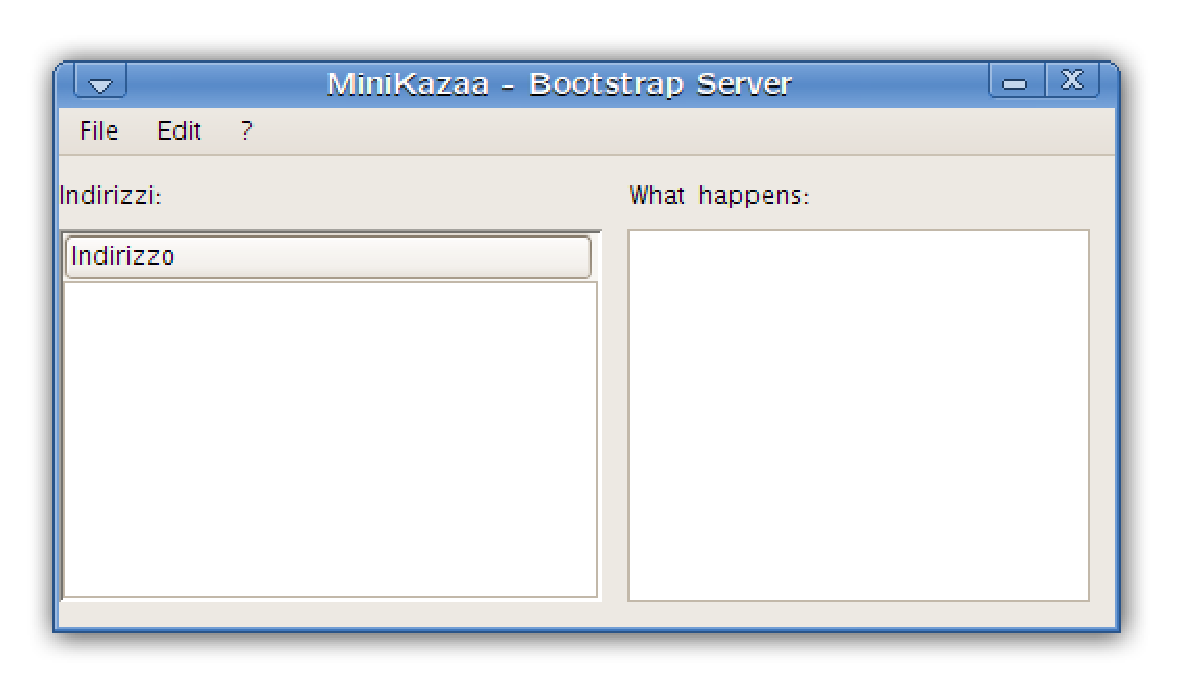
\includegraphics[width=300px,height=160px]{images/bss_grafica.eps}
 % bss_grafica.eps: 0x0 pixel, 300dpi, 0.00x0.00 cm, bb=14 14 564 329
 \caption{Interfaccia grafica del Bootstrap server}
 \label{fig:bss_grafica}
\end{figure}

Uno screenshot dell'interfaccia grafica principale del Bootstrap server si può vedere in Figura \ref{fig:bss_grafica}.

Nella parte a sinistra dell'interfaccia vengono inseriti gli \emph{id} di tutti i nodi che si connettono alla rete.

Nella parte destra, invece, vengono visualizzati dei messaggi che spiegano cosa avviene all'iterno della rete.




\end{document}
